\documentclass[10pt]{beamer}
\usepackage[utf8]{inputenc}
\usepackage[T1]{fontenc}
\usepackage[english]{babel}
\usepackage{graphicx}
\usepackage{caption}
\usepackage{xcolor}
\usepackage{hyperref}
% https://www.hartwork.org/beamer-theme-matrix/
\usetheme{Warsaw}

% Modify Warshaw theme. Make it dark.
\setbeamercolor{normal text}{fg=white,bg=black!90}
\setbeamercolor{structure}{fg=white}

\setbeamercolor{alerted text}{fg=red!85!black}

\setbeamercolor{item projected}{use=item,fg=black,bg=item.fg!35}

\setbeamercolor*{palette primary}{use=structure,fg=structure.fg}
\setbeamercolor*{palette secondary}{use=structure,fg=structure.fg!95!black}
\setbeamercolor*{palette tertiary}{use=structure,fg=structure.fg!90!black}
\setbeamercolor*{palette quaternary}{use=structure,fg=structure.fg!95!black,bg=black!80}

\setbeamercolor*{framesubtitle}{fg=white}

\setbeamercolor*{block title}{parent=structure,bg=black!60}
\setbeamercolor*{block body}{fg=black,bg=black!10}
\setbeamercolor*{block title alerted}{parent=alerted text,bg=black!15}
\setbeamercolor*{block title example}{parent=example text,bg=black!15}

% By default beamer puts all items right next to each other,
% this spaces them out a bit.
% To use uncomment the lines below.
\newlength{\wideitemsep}
\setlength{\wideitemsep}{\itemsep}
    \addtolength{\wideitemsep}{10pt}
\let\olditem\item
\renewcommand{\item}{\setlength{\itemsep}{\wideitemsep}\olditem}

% Include minted and choose a colorscheme
\usepackage{minted}
% pygmentize -L styles
% pygmentize -L lexers
\usemintedstyle{monokai}

% Customize the display style of line numbers
\renewcommand{\theFancyVerbLine}{\sffamily
    \textcolor[rgb]{0.5,0.5,1.0}{\scriptsize
    \oldstylenums{\arabic{FancyVerbLine}}}}
% http://latexcolor.com/
\definecolor{lightskyblue}{rgb}{0.53, 0.81, 0.98}

% Configure the behaviour of the links
\hypersetup{
    colorlinks = true,
    linkcolor = white,
    urlcolor = lightskyblue,
    filecolor = white,
    pdfkeywords = {code, mathematics, physics},
    pdfauthor = {\author},
    pdftitle = {\title},
    pdfsubject = {Beamer},
    pdfpagemode = UseNone, %FullScreen
}

% Information to be included in the title page:
\title{Sample title}
\author{Anonymous}
\institute{Faculty of Physics\\
  Very Famous University}
\date{\today}

\begin{document}

\frame{\titlepage}

% Input code from a file. Use [fragile] to render correctly
\begin{frame}[fragile]
\frametitle{K\&R Hello World}
\inputminted{c}{hello.c}
\end{frame}

\begin{frame}[fragile]
    \frametitle{99 Bottles of Beer}
\begin{minted}[linenos=true]{befunge}
<v  <.g10" bottles of beer on the wall"+*4310     <
c>:,|
    <v  <.g10" bottles of beer"+*4310
     >:,|
        <v  <"take one down, pass it around"+*4310
         >:,|
            >01g1-:01p                      v
v  <.g10" bottles of beer on the wall"+*4310<
>:,|
   >134*+0`                                       |
\end{minted}
\end{frame}

\begin{frame}
\frametitle{One-line code}
\begin{itemize}
\item One-line code formatting sample: 
\mint{tex}|{\mint{tex}|x \Rightarrow y|}|
\item A html example:
\mint{html}|<p>Sample <strong>text</strong></p>|
\end{itemize}
\end{frame}

\begin{frame}
\frametitle{Sample frame title}
 
In this slide, some important text will be
\alert{highlighted} beause it's important.
Please, don't abuse it.
 
\begin{block}{Remark}
Sample text
\end{block}
 
\begin{alertblock}{Important theorem}
Sample text in red 
\end{alertblock}
 
\begin{examples}
Sample text in green. "Examples" is fixed as block title.
\end{examples}
\end{frame}

{
\begin{frame}
\frametitle{Sample frame title}
 In this slide \pause
 
 the text will be partially visible \pause
 
 And finally everything will be there
\end{frame}
}

\begin{frame}
\frametitle{Sample frame title}
This is a text in second frame. 
For the sake of showing an example.
 
\begin{itemize}
 \item<1-> Text visible on slide 1
 \item<2-> Text visible on slide 2
 \item<3> Text visible on slide 3
 \item<4-> Text visible on slide 4
\end{itemize}
\end{frame}

\begin{frame}
\frametitle{Two-column slide}
 
\begin{columns}
 
\column{0.5\textwidth}
This is a text in first column.
$$E=mc^2$$
\begin{itemize}
\item First item
\item Second item
\end{itemize}
 
\column{0.5\textwidth}
This text will be in the second column
and on a second tought this is a nice looking
layout in some cases.
\end{columns}
\end{frame}

{
\usebackgroundtemplate{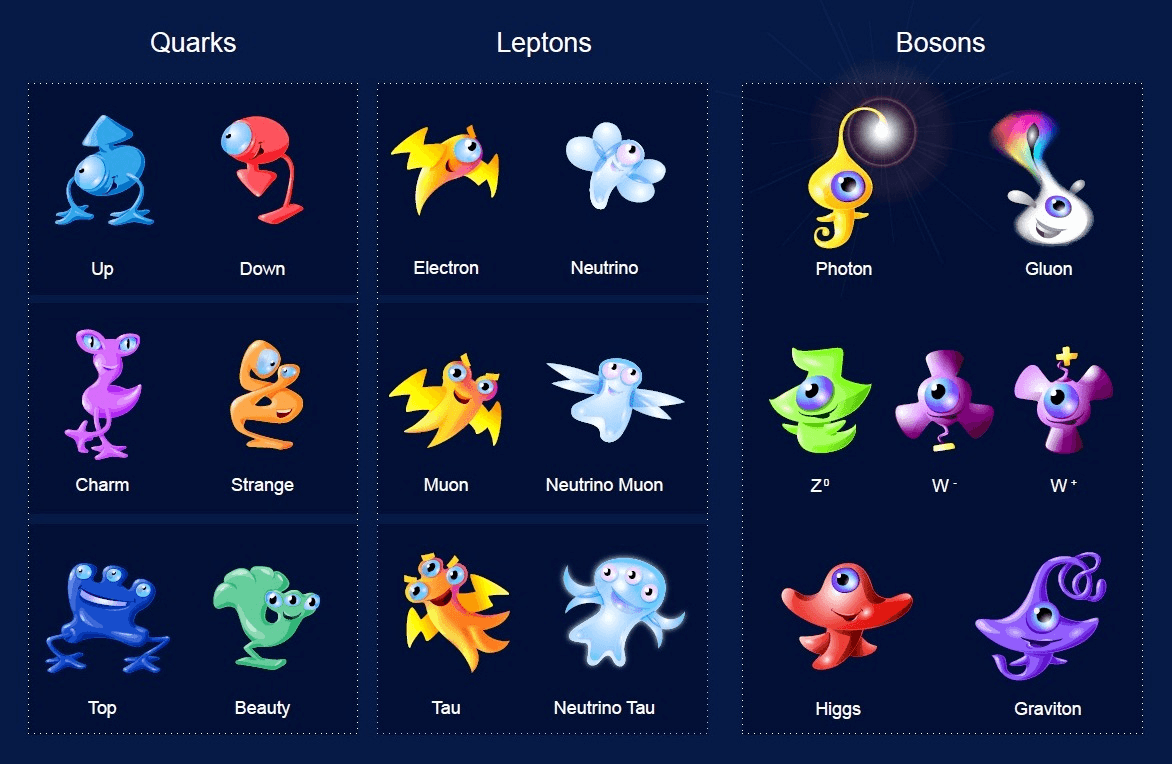
\includegraphics[width=\paperwidth,height=\paperheight,clip]{Sprites.png}}
\frame{
\frametitle{Backround Image}
%Text here
}
}

\begin{frame}
\frametitle{Sample equation}
\begin{gather}\label{eq:1}
ds^2=c^2dt^2-R^2(t)\left\{\frac{d\sigma^2+\sigma^2(d\theta^2+\sin^2\theta d\phi^2)}
    {\left[(1+\frac{k}{4})\sigma^2\right]^2}\right\}\:
\end{gather}
\end{frame}

\begin{frame}[fragile]
\frametitle{The End}
\begin{columns}

\column{0.5\textwidth}
\begin{minted}{asm}
mov ebx,    0
mov eax,    1
int 0x80
\end{minted}
\par
\vspace{2em}
Homepage: \href{http://example.com}{\tt example.com}\\
Email: \href{mailto:some@example.com}{\tt some@example.com}

\column{0.5\textwidth}
\begin{figure}[ht]
    
\includegraphics[width=0.5\textwidth]{insect.png}
    \caption{\href{https://twitter.com/Pixel_Dailies}{Pixel Dailies}}
\end{figure}
\end{columns}
\end{frame}  

\end{document}


